\documentclass[12pt, letterpaper]{article} 
\usepackage[utf8]{inputenc}
\usepackage{setspace}
\usepackage[spanish]{babel} %pone en español textos automaticos
\usepackage{fancyhdr} % Se agrega el paquete fancyhdr
\usepackage{graphicx} % Se agrega el paquete graphicx
\usepackage[a4paper, margin=3cm]{geometry} %marjenes y hoja A4


%pies de pagina.
\pagestyle{fancy} % Se especifica el estilo de página como fancy
\fancyhf{} % Se limpian los encabezados y pies de página predefinidos
\rfoot{Página \thepage\ de \pageref{LastPage}} %texto derecha
\lfoot{Electronica Aplicada II} %texto izquierda
%encabezado de pagina
\chead{UNIVERSIDAD TECNOLÓGICA NACIONAL - FRC} % centro
\fancyhead[R]{
\includegraphics[height=1cm]{Imagenes/UTN_logo.jpg}}


\begin{document}

%Caratula
\begin{titlepage}
	\centering %texto centrado
	{
\includegraphics[width=0.2\textwidth]{Imagenes/UTN_logo.jpg}\par}
	{\bfseries\LARGE Universidad Tecnológica Nacional \par}
	{\scshape\Large Facultad Regional Córdoba\par}
	\vspace{1cm}
	{\scshape\Huge Amplificador Realimentado V-S \par}%titulo
	\raggedright %texto a la izquierda
	\vspace{1cm}
	{\Large Materia: Electronica Aplicada II \par}%Materia
	\vspace{0.5cm}
	{\Large Curso: 4R1 \par}
	\vspace{0.5cm}
	{\Large Edificio: \par}%edificios
	\begin{itemize}
		\item{\Large Ingeniero Soro [Aula 606] \par}
		\item{\Large Laboratorio de electrónica \par}
	\end{itemize}
	\vspace{0.5cm}
	{\Large Profesores: \par} %profes
	\begin{itemize}
		\item{\Large [Teórico] Ing, Carlos Celdran \par}
		\item{\Large [Teórico] Ing, Carlos Enrique Olmos \par}
		\item{\Large [Práctico] Ing, Federico Luis José Linares \par}
	\end{itemize}
	\vspace{0.5cm}
	{\Large Autores: \par} %autores
	\begin{itemize}
		\item{\Large Pappano Meinardi, Joaquín - Leg.86730\par}
		\item{\Large Monteros Vigueras, Juan Manuel - Leg.86334\par}
		\item{\Large Romero Diaz, Agustín - Leg.86821\par}
	\end{itemize}
	\vspace{0.5cm}
	{\Large Fecha: {\today} \par}%pone fecha de hoy
\end{titlepage}

%Indice
\newpage
\tableofcontents
\newpage

%cuerpo documento
\section{Introducción}

La retroalimentación negativa es una técnica ampliamente utilizada en el diseño de circuitos electrónicos para mejorar la estabilidad, la linealidad y la precisión de los amplificadores.
El amplificador de retroalimentación negativa V-S es un ejemplo común de esta técnica, que utiliza una red beta y un amplificador multietapas para reducir la ganancia y mejorar la linealidad del circuito.
En este informe, se presentará una descripción detallada del diseño y funcionamiento del amplificador de retroalimentación negativa V-S, así como su análisis teórico y experimental.
Además, se discutirán algunas de las aplicaciones prácticas de este tipo de amplificador en la electrónica analógica y su ancho de banda.

\section{Cálculos Teóricos}
Se realizaron los cálculos de $A_v$, $Z_o$, $Z_i$, $A_{vf}$, $Z_{of}$, $Z_{if}$
\singlespacing
Estamos frente a un amplificador el cual tiene unas función de transferencia $H(s)=\frac{V_o}{V_i}
$ por lo tanto el circuito equivalente de este lo podemos ver en la figura \ref{fig:2.1}
\begin{figure}[h]
	\centering
	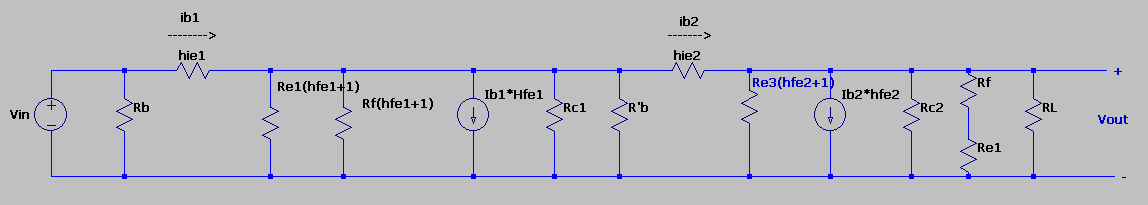
\includegraphics[width=0.75\textwidth]{Imagenes/circeq.png}
	\caption{Circuito equivalente amplificador realimentado V-S}
	\label{fig:2.1}
\end{figure}
\singlespacing
definiremos los parámetros de este circuito respecto al esquemático dado
\singlespacing
$R_B=R_{b1}//R_{b2} \rightarrow 332K8\Omega$\hspace{1cm} 
\singlespacing
$R_{e3} \rightarrow 240\Omega$\hspace{1cm} $R_{L} \rightarrow 470\Omega$ \hspace{1cm} $R_{f} \rightarrow 1k6\Omega$
\singlespacing
$Rf \rightarrow 1K6\Omega$ \hspace{1cm} $R_B'=R_{b3}//R_{b4} \rightarrow 19K7\Omega$ \hspace{1cm} $R_{c1} \rightarrow18K\Omega$
\singlespacing
$hfe1 \rightarrow 359$ \hspace{1cm} $hfe2 \rightarrow 339$ $R_{c2} \hspace{1cm} \rightarrow 2K\Omega$
\singlespacing
Para $hie$ se deben encontrar las corriente ICQ1 e ICQ2 Para eso analizarimos la polarizacion de los traacitores
\\
\begin{figure}[h]
	\centering
	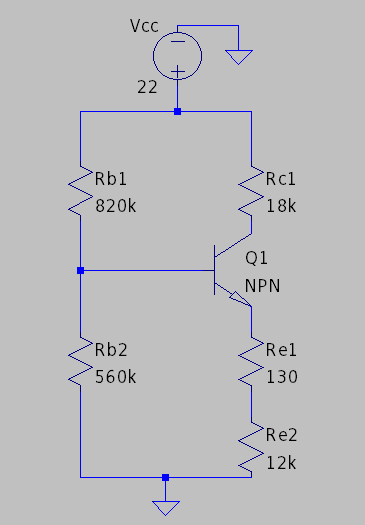
\includegraphics[width=0.75\textwidth]{Imagenes/polarizacionQ1.png}
	\caption{Polarizacion Q1}
	\label{fig:2.4}
\end{figure}
$Vcc-VR_{b1}-VR_{b2}=0 \rightarrow ICQ1=hfe1\frac{Vcc}{R_{b1}+R_{b2}}=5,73mA$
\\
$hie1=hfe1\frac{25mV}{ICQ1}=1568\Omega$
\\
\begin{figure}[h]
	\centering
	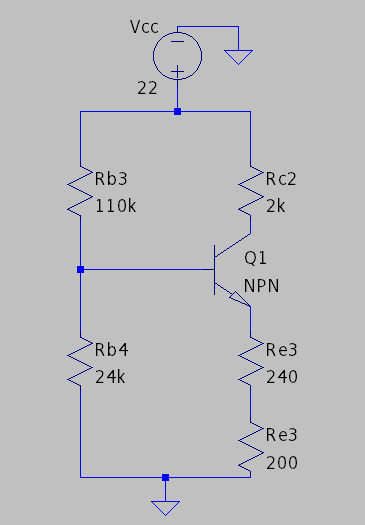
\includegraphics[width=0.75\textwidth]{Imagenes/PolarizaQ2.png}
	\caption{Polarizacion Q2}
	\label{fig:2.5}
\end{figure}
$Vcc-VR_{b3}-VR_{b4}=0 \rightarrow ICQ2=hfe2\frac{Vcc}{R_{b3}+R_{b4}}=55,65mA$
\\
$hie2=hfe2\frac{25mV}{ICQ2}=152\Omega$
\\

Las ecuaciones que podemos obtener del análisis del circuito son
\singlespacing
$i_{b1}=V_i\frac{1}{hie_1+[(R_{e1}//R_f)(hfe + 1)]} \rightarrow \frac{i_{b1}}{v_i}=\frac{1}{hie_1+[(R_{e1}//R_f)(hfe + 1)]}=22,36*10^{-6}$
\singlespacing
$ i_{b2}=ib1(-hfe\frac{R_{e1}//R_b'//(hie_2+R_{e3}(hfe_2+1))}{(hie_2+R_{e3}(hfe_2+1))}{hie_2})}) \rightarrow \frac{i_{b2}}{i_{b1}}=-hfe\frac{R_{e1}//R_b'//(hie_2+R_{e3}(hfe_2+1))}{(hie_2+R_{e3}(hfe_2+1))}{hie_2})}=35$
\singlespacing
$V_o=i_{b2}(-hfe[R_{e2}//(R_f+R_{e2})]) \rightarrow \frac{V_o}{i_{b2}}=-hfe[R_{e2}//(R_f+R_{e2}]=105749$
\subsection{Calculo Av}
$A_v=\frac{V_o}{V_i}=\frac{v_o}{i_{b2}}\frac{i_{b2}}{i_{b1}}\frac{i_{b1}}{v_i}=82,87$
\subsection{Calculo Red beta y calculo Avf}
\begin{figure}[h]
	\centering
	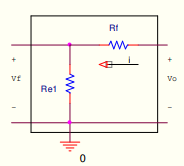
\includegraphics[width=0.75\textwidth]{Imagenes/Screenshot_58.png}
	\caption{Red Beta  V-S}
	\label{fig:2.2.1}
\end{figure}
\singlespacing
$v_o=i(R_f+R_{e1})$ \hspace{1cm} $vf=iR_{e1}$
\singlespacing
$\beta = \frac{v_f}{v_o}=\frac{R_{e1}}{R_{e1}+R_f}=0,075$
\singlespacing
$D=|1+A_v\beta|=7,1618$ \hspace{1cm} $A_{vf}=\frac{A_v}{D}=11,57$
\subsection{Cálculos de Zi,Zo,Zif,Zof}
Lazo abierto:
$Z_i=R_b//{hie_1+[(R_{e1}//R_f)(hfe+1)]}=39523\Omega$
\singlespacing
$Z_o=R_{c2}//(R_{e1}+R_f)=927,61\Omega$
\singlespacing
Lazo cerrado :
$Z_{if}=Z_i*D=283K\Omega$
\singlespacing
$Z_{of}=\frac{Z_o}{D}=130\Omega$
\section{Simulaciones}

\section{Procedimiento}
\subsection{Consignas Solitadas}
\begin{itemize}
	\item  Implementar un amplificador realimentado
    \item  Realizar las mediciones $A_v, Z_o,Z_i, A_{vf},Z_{of},Z_{if} $
    \item  Realizar la medición de Desensibilidad provocando una variación máxima de Av del 45%, para lo
	cual se deberá modificar algún componente del amplificador (usaremos Re3).
    \item Obtener y graficar la curva de respuesta en frecuencia de la ganancia circuito a lazo abierto y lazo
	cerrado del circuito implementado. Para esto se utilizará los generadores provistos por el
	laboratorio centra
    \item Haciendo uso del simulador verificar los valores obtenidos del punto anterior (ganancia y
	respuesta en frecuencia).
\end{itemize}
Para poder realizar las mediciones solicitadas , se realizo el pcb del circuito correspondiente y se monto los componentes en el mismo.
Una vez hecho esto se alimeto el circuito con 22V C.C, en paralelo con $R_L$ se conecto un osiloscopio digital para poder medir la salida y en la entrada un generador de ondas $V_{in}= 60 V_{pp}$ como en el esquema de figura \ref{fig:4.1}
\begin{figure}[h]
	\centering
	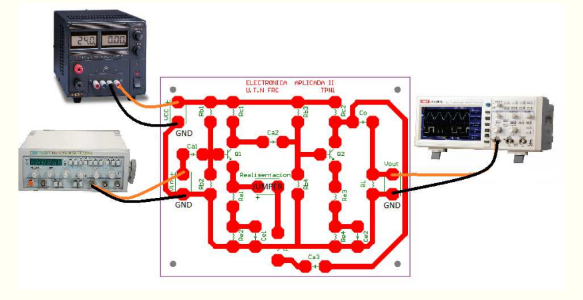
\includegraphics[width=0.75\textwidth]{Imagenes/conexion.png}
	\caption{Conexiones amplificador realimentado V-S}
	\label{fig:4.1}
\end{figure}
\subsection{Mediciones}
Se comenzo midiendo la salida a lazo abierto $V_o=4V_{pp}$, se procedio a conectar la realimentacion a la salida y se obtuvo la $V_o=700mV$ a lazo cerrado
\singlespacing
$A_{v1}=\frac{V_o}{V_{i}}=\frac{4V}{0.06V}=66.66\therefore A_{vf1}=\frac{V_o}{V_{i}}=\frac{700mV}{60mV}=11.66$
\singlespacing
Para reducir la ganacia a lazo abierto un 45 \% se remplazo $R_{e3}$ por un tripo de $1K\Omega$ y se lo vario hasta que la $V_o=2,2V$ en lazo abierto esto se logro con el tripo en $500\omega$, se conecto la realimentacio en se midio $V_o=550mv$
\singlespacing
Con estos datos se volvio a calcular $A_{v2}=\frac{V_o}{V_{i}}=\frac{2,2V}{0.06V}=36.66\therefore A_{vf2}=\frac{V_o}{V_{i}}=\frac{550mV}{60mV}=9.66$
\singlespacing
$D=\frac{\Delta \% A_v}{\Delta \% A_{vf}}=\frac{45\%}{21,44\%}=2,09$
\singlespacing
Una vez calculada la desensibilidad se conecto en la entrada un tripo de $100k\Omega$ con se muestra en la figura\ref{fig:4.2}
\singlespacing
\begin{figure}[h]
	\centering
	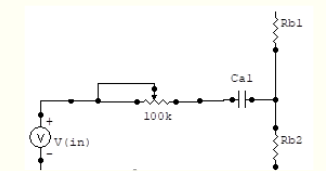
\includegraphics[width=0.75\textwidth]{Imagenes/zi.png}
	\caption{Circuito para medicion Zi}
	\label{fig:4.2}
\end{figure}
con el amplificador a lazo abierto se aumento la $V_i$ hasta llegar al punto MES(Maxima excurcion simetrica) $V_o=4,8V$, se conecto el tripo y se lo vario hasta llegar a una $V_o=2,4V$, se saco el tripo y se lo medio
\singlespacing
$Z_i=40,26k\Omega$
\singlespacing
Para $Z_o$ se realizo la conexion de la figuta\ref{fig:4.3}
\singlespacing
\begin{figure}[h]
	\centering
	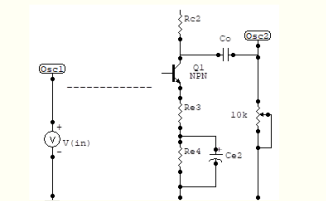
\includegraphics[width=0.75\textwidth]{Imagenes/zo.png}
	\caption{Circuito para medicion Zo}
	\label{fig:4.3}
\end{figure}
\label{LastPage}
\end{document}